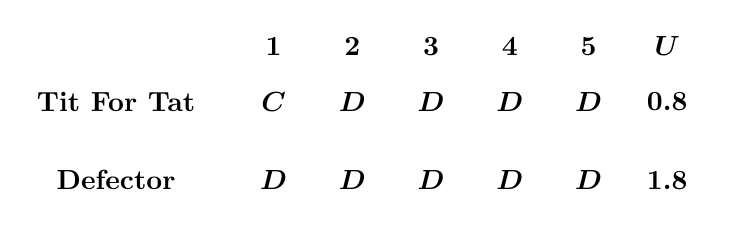
\begin{tikzpicture}
    
    \tikzstyle{state}=[minimum width=1cm, font=\boldmath];
    

    \node[thick] (0) at (-1, 0) [state] {\textbf{Tit For Tat}};
    \node[thick] (1) at (-1, -1) [state] {\textbf{Defector}};

    \node[thick] (2) at (1, 0.7) [state] {$1$};
    \node[thick] (3) at (2, 0.7) [state] {$2$};
    \node[thick] (4) at (3, 0.7) [state] {$3$};
    \node[thick] (5) at (4, 0.7) [state] {$4$};
    \node[thick] (6) at (5, 0.7) [state] {$5$};
    \node (8) at (1, 0) [state] {$C$};
    \node (14) at (1, -1) [state] {$D$};
    \node (9) at (2, 0) [state] {$D$};
    \node (10) at (3, 0) [state] {$D$};
    \node (15) at (2, -1) [state] {$D$};
    \node (16) at (3, -1) [state] {$D$};
    \node (11) at (4, 0) [state] {$D$};
    \node (17) at (4, -1) [state] {$D$};
    \node (12) at (5, 0) [state] {$D$};
    \node (18) at (5, -1) [state] {$D$};


    \node[thick] (7) at (6, 0.7) [state] {$U$};
    \node (13) at (6, 0) [state] {$0.8$};
    \node (19) at (6, -1) [state] {$1.8$};

        % \node [background, fit=(14) (15) (16)] {};


    \end{tikzpicture}